% Copyright © 2015
% Eduardo Candido Xavier <eduardo@ic.unicamp.br>
%
% This work is free. You can redistribute it and/or modify it under the
% terms of the Do What The Fuck You Want To Public License, Version 2,
% as published by Sam Hocevar. See the COPYING file for more details.
%
% DO WHAT THE FUCK YOU WANT TO PUBLIC LICENSE
% Version 2, December 2004
%
% Copyright (C) 2004 Sam Hocevar <sam@hocevar.net>
%
% Everyone is permitted to copy and distribute verbatim or modified
% copies of this license document, and changing it is allowed as long
% as the name is changed.
%
% DO WHAT THE FUCK YOU WANT TO PUBLIC LICENSE
% TERMS AND CONDITIONS FOR COPYING, DISTRIBUTION AND MODIFICATION
%
% 0. You just DO WHAT THE FUCK YOU WANT TO.

\documentclass[handout]{beamer}
\usetheme{metropolis}
\beamertemplatetransparentcoveredhigh

\usepackage[portuges]{babel}
\usepackage{graphicx}
\graphicspath{{./figs/}}
\usepackage{listings}
\usepackage{color}
\usepackage{hyperref}
\usepackage{xpatch}
\usepackage{amsmath}
\usepackage[outputdir=build]{minted}

\makeatletter
\AtBeginEnvironment{minted}{\dontdofcolorbox}
\def\dontdofcolorbox{\renewcommand\fcolorbox[4][]{##4}}
\xpatchcmd{\inputminted}{\minted@fvset}{\minted@fvset\dontdofcolorbox}{}{}
\xpatchcmd{\mintinline}{\minted@fvset}{\minted@fvset\dontdofcolorbox}{}{}
\makeatother
\setminted[c]{
  linenos=true,
  breaklines=true,
  encoding=utf8,
  frame=lines,
  framerule=0.5pt,
  autogobble,
  fontsize=\small,
}
\setminted[bash]{
  linenos=true,
  encoding=utf8,
  frame=lines,
  framerule=0.5pt,
  autogobble,
  fontsize=\small
}

\newcommand{\cod}[1]{\mintinline{c}{#1}}


\definecolor{dkgreen}{rgb}{0,0.6,0}
\definecolor{gray}{rgb}{0.5,0.5,0.5}
\definecolor{mauve}{rgb}{0.58,0,0.82}


\definecolor{Purple}{HTML}{911146}
\definecolor{Orange}{HTML}{CF4A30}
\setbeamercolor{alerted text}{fg=Orange}
\setbeamercolor{frametitle}{bg=Purple}
\setbeamercolor{block body}{bg=Purple!20,fg=black}
\setbeamercolor{block title}{bg=Purple!50,fg=black}
\setbeamertemplate{blocks}[rounded][shadow=true]


\newcommand{\setcoverbg}{
  \setbeamertemplate{background}
  {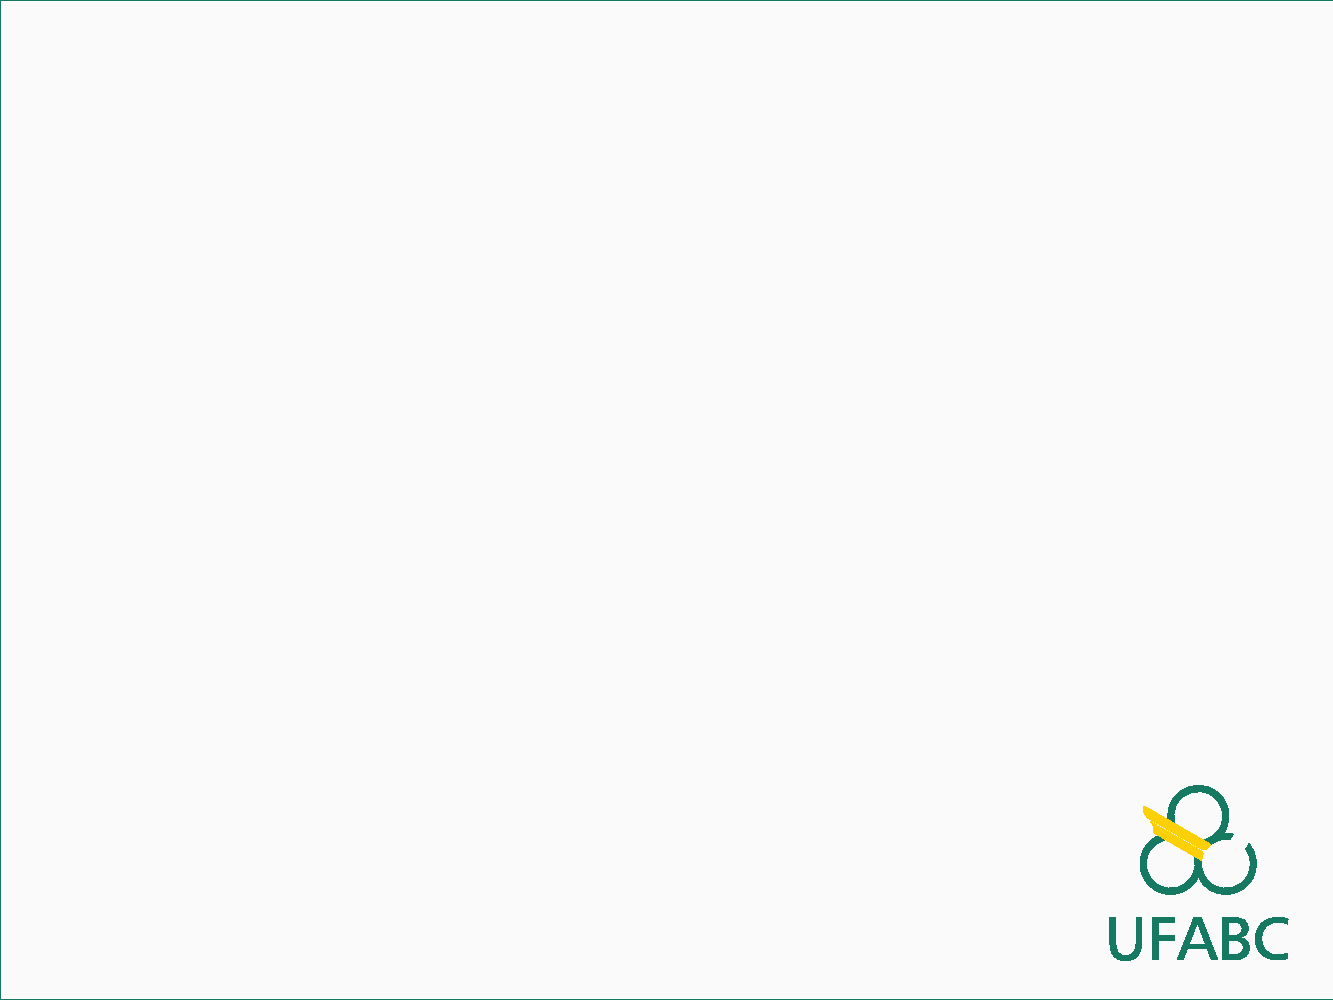
\includegraphics[width=\paperwidth,height=\paperheight]{backgrounds/coverbg}}
}
\newcommand{\setsectionbg}{
  \setbeamertemplate{background}
  {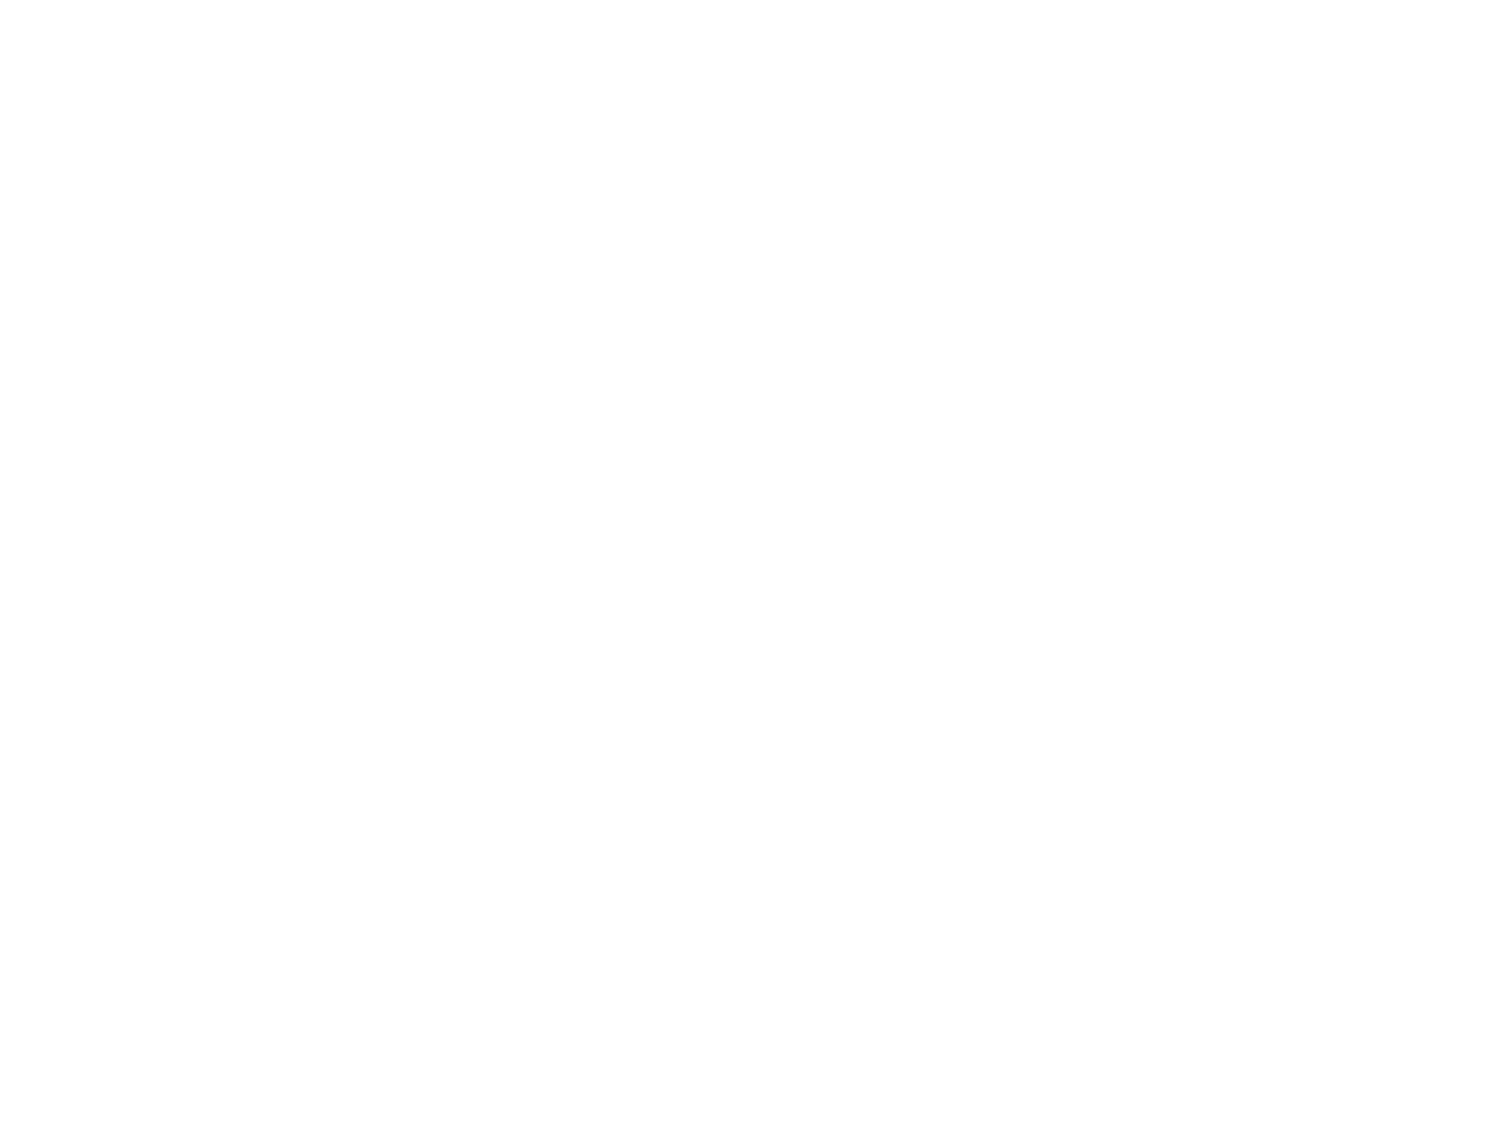
\includegraphics[width=\paperwidth,height=\paperheight]{backgrounds/blank}}
}

\title{Programação Estruturada}
\subtitle{Recursão}

\author{Professores Emílio Francesquini e Carla Negri Lintzmayer}
\institute{Centro de Matemática, Computação e Cognição\\ Universidade Federal do ABC}
\date{2018.Q3}

\begin{document}

\setcoverbg
\maketitle
\setsectionbg

%%%%%%%%%%%%%%%%%%%%%%%%%%%%%%%%%%%%%%%%%%%%%%%%%%%%%%%%%%%%%%
%%%%%%%%%%%%%%%%%%%%%%%%%%%%%%%%%%%%%%%%%%%%%%%%%%%%%%%%%%%%%%
%%%%%%%%%%%%%%%%%%%%%%%%%%%%%%%%%%%%%%%%%%%%%%%%%%%%%%%%%%%%%%
%%%%%%%%%%%%%%%%%%%%%%%%%%%%%%%%%%%%%%%%%%%%%%%%%%%%%%%%%%%%%%
%%%%%%%%%%%%%%%%%%%%%%%%%%%%%%%%%%%%%%%%%%%%%%%%%%%%%%%%%%%%%%
%%%%%%%%%%%%%%%%%%%%%%%%%%%%%%%%%%%%%%%%%%%%%%%%%%%%%%%%%%%%%%

\section{Recursão}

%%%%%%%%%%%%%%%%%%%%%%%%%%%%%%%%%%%%%%%%%%%%%%%%%%%%%%%%%%%%%%
\begin{frame}{Recursão}
    \centering
    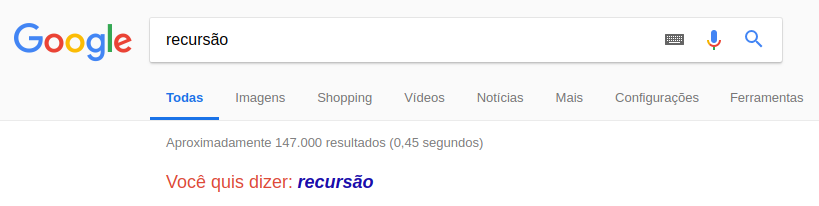
\includegraphics[width=\textwidth]{figs/recursao-google}
\end{frame}

%%%%%%%%%%%%%%%%%%%%%%%%%%%%%%%%%%%%%%%%%%%%%%%%%%%%%%%%%%%%%%
\begin{frame}{Recursão}
    \centering
    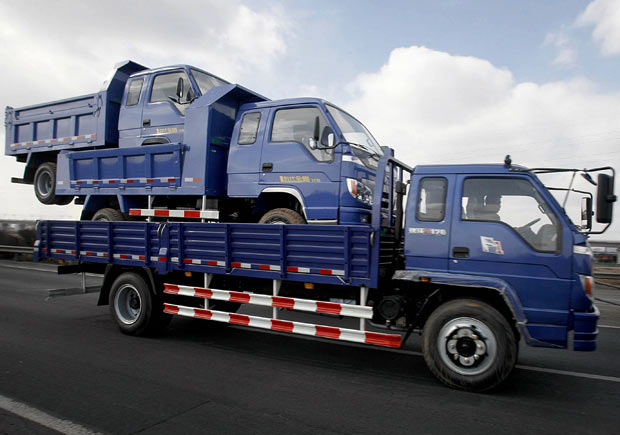
\includegraphics[width=\textwidth]{figs/trucks}
\end{frame}

%%%%%%%%%%%%%%%%%%%%%%%%%%%%%%%%%%%%%%%%%%%%%%%%%%%%%%%%%%%%%%
\begin{frame}{Recursão}
  O que os seguintes problemas têm em comum?
  \begin{itemize}

    \item \textbf{Fatorial}
    \begin{equation*}
      F_i =
      \begin{cases}
        1                & \text{se } i = 0 \\
        i \times F_{i-1} & \text{caso contrário}
      \end{cases}
    \end{equation*}

    \item  O $i$-ésimo elemento da \textbf{Sequência de
    Fibonacci ($F_i$)}
    \begin{equation*}
      F_i =
      \begin{cases}
        i                 & \text{se } i < 2 \\
        F_{i-1} + F_{i-2} & \text{caso contrário}
      \end{cases}
    \end{equation*}

    \item Máximo divisor comum (\textbf{MDC})
    \begin{equation*}
      MDC(a, b) =
      \begin{cases}
        a                        & \text{se } b = 0 \\
        MDC(b, a~\mathrm{mod}~b) & \text{caso contrário}
      \end{cases}
    \end{equation*}

  \end{itemize}
\end{frame}

%%%%%%%%%%%%%%%%%%%%%%%%%%%%%%%%%%%%%%%%%%%%%%%%%%%%%%%%%%%%%%
\begin{frame}[fragile]{Recursão}
  \begin{itemize}
    \item \textbf{Fatorial}
    \begin{minted}[fontsize=\scriptsize]{c}
      int fatorial(int i) {
          if (i == 0) return 1;
          return i * fatorial(i - 1);
      }
    \end{minted}

    \item  O $i$-ésimo elemento da \textbf{Sequência de
    Fibonacci ($F_i$)}
    \begin{minted}[fontsize=\scriptsize]{c}
      int fib(int i) {
          if (i < 2) return i;
          return fib(i - 1) + fib(i - 2);
      }
    \end{minted}
    \item Máximo divisor comum (\textbf{MDC})
    \begin{minted}[fontsize=\scriptsize]{c}
      int mdc(int a, int b) {
          if (b == 0) return a;
          return mdc(b, a % b);
      }
    \end{minted}
  \end{itemize}
\end{frame}

%%%%%%%%%%%%%%%%%%%%%%%%%%%%%%%%%%%%%%%%%%%%%%%%%%%%%%%%%%%%%%
\begin{frame}{Recursão}

    \begin{itemize}[<+->]
        \item Um objeto é denominado recursivo quando sua definição é parcialmente feita em termos dele mesmo.
        \item Em programação, a recursividade é um mecanismo útil e poderoso que permite a uma função chamar a si mesma direta ou indiretamente.
        \item A ideia básica de um algoritmo recursivo consiste em diminuir sucessivamente o problema em um problema menor ou mais simples, até que o possamos resolver o problema reduzido de forma direta.
        \begin{itemize}
            \item Quando isso ocorre, atingimos uma \textbf{condição de parada}.
        \end{itemize}
    \end{itemize}
\end{frame}

%%%%%%%%%%%%%%%%%%%%%%%%%%%%%%%%%%%%%%%%%%%%%%%%%%%%%%%%%%%%%%
%%%%%%%%%%%%%%%%%%%%%%%%%%%%%%%%%%%%%%%%%%%%%%%%%%%%%%%%%%%%%%
%%%%%%%%%%%%%%%%%%%%%%%%%%%%%%%%%%%%%%%%%%%%%%%%%%%%%%%%%%%%%%
%%%%%%%%%%%%%%%%%%%%%%%%%%%%%%%%%%%%%%%%%%%%%%%%%%%%%%%%%%%%%%
%%%%%%%%%%%%%%%%%%%%%%%%%%%%%%%%%%%%%%%%%%%%%%%%%%%%%%%%%%%%%%
%%%%%%%%%%%%%%%%%%%%%%%%%%%%%%%%%%%%%%%%%%%%%%%%%%%%%%%%%%%%%%

\section{Indução}

%%%%%%%%%%%%%%%%%%%%%%%%%%%%%%%%%%%%%%%%%%%%%%%%%%%%%%%%%%%%%%
\begin{frame}[fragile]{Indução}

    \begin{center}
        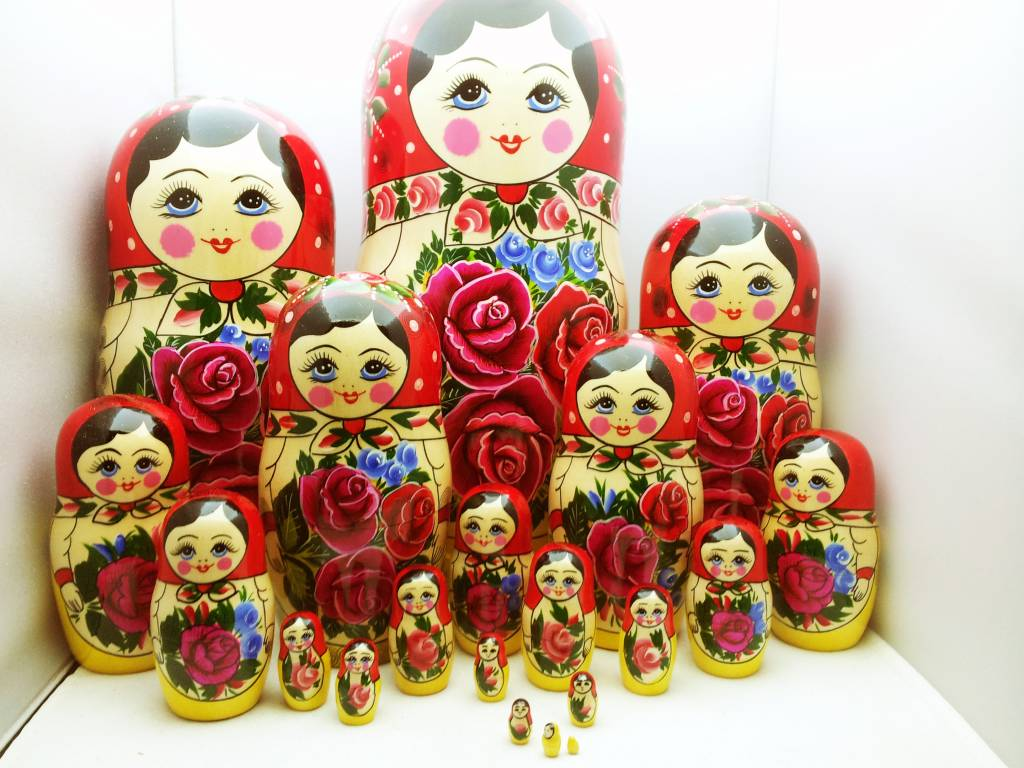
\includegraphics[width=0.5\textwidth]{figs/matrioska}
    \end{center}

    \begin{itemize}[<+->]
        \item Usando o método de indução, a solução de um problema pode ser expressa da seguinte forma:
        \begin{itemize}
            \item Primeiramente, definimos a solução para casos básicos;
            \item Em seguida, definimos como resolver o problema para um caso geral, utilizando-se de soluções para instâncias menores do problema.
        \end{itemize}
    \end{itemize}
\end{frame}

%%%%%%%%%%%%%%%%%%%%%%%%%%%%%%%%%%%%%%%%%%%%%%%%%%%%%%%%%%%%%%
\begin{frame}[fragile]{Indução}

    \begin{itemize}[<+->]
        \item {\bf Indução:} Técnica de demonstração matemática onde algum parâmetro da proposição a ser demonstrada envolve números naturais.
        \item Seja $T(n)$ uma proposição que desejamos provar como verdadeira para todos valores naturais $n$.
        \item Ao invés de provar diretamente que $T(n)$ é válida para todos os valores de $n$, basta:
        \begin{enumerate}
            \item {\bf Caso base:} Provar que $T(1)$ é válido.
            \item {\bf Hipótese de Indução:} Assumir que $T(n-1)$ é válida.
            \item {\bf Passo de indução:} Provar que $T(n)$ é válida.
        \end{enumerate}
    \end{itemize}
\end{frame}

%%%%%%%%%%%%%%%%%%%%%%%%%%%%%%%%%%%%%%%%%%%%%%%%%%%%%%%%%%%%%%
\begin{frame}[fragile]{Indução}

    \begin{itemize}
        \item Por que a indução funciona?
        \begin{itemize}
            \item Mostramos que $T(1)$ é valida.
            \item Com o passo da indução, automaticamente mostramos que $T(2)$ é válida.
            \item Como $T(2)$ é válida, pelo passo de indução, $T(3)$ também é válida.
            \item E assim por diante\ldots
        \end{itemize}
    \end{itemize}
\end{frame}

%%%%%%%%%%%%%%%%%%%%%%%%%%%%%%%%%%%%%%%%%%%%%%%%%%%%%%%%%%%%%%
\begin{frame}[fragile]{Indução}

    \begin{itemize}
        \item {\bf OBS:} O caso base não precisa ser necessariamente com $n=1$.
        \item Você pode considerar um caso inicial $n=c$ para uma constante $c$ qualquer.
        \item Se você mostrar que este caso base é valido e o passo também é valido: sua proposição é verdadeira para todo $n \geq c$.
    \end{itemize}
\end{frame}

%%%%%%%%%%%%%%%%%%%%%%%%%%%%%%%%%%%%%%%%%%%%%%%%%%%%%%%%%%%%%%
\begin{frame}[fragile]{Exemplo}

    \begin{block}{Teorema}
        $2^{2n}-1$ é múltiplo de 3 para $n \geq 0$.
    \end{block}

    \pause
    {\bf Base:} Para $n=0$ temos que $2^{2n} -1 = 0$, que é múltiplo de 3.

    \pause
    {\bf Hipótese:} O teorema é válido para $n-1$, ou seja, $2^{2(n-1)}-1$ é múltiplo de 3.

    \pause
    {\bf Passo:} Devemos provar que $2^{2n} -1$ é múltiplo de 3.
    Para tanto, vamos usar a hipótese.
    \pause
    Note que $$2^{2n} -1 = 2^{2n-2}2^{2}-1=4(2^{2(n-1)}) -1 = 3(2^{2(n-1)}) + 2^{2(n-1)} -1.$$
    \pause
    Note que $3(2^{2(n-1)})$ é múltiplo de 3 e, por hipótese, $2^{2(n-1)} -1$ também é múltiplo de 3.
    \pause
    Portanto, $$3(2^{2(n-1)}) + 2^{2(n-1)} -1 = 2^{2n} -1$$ é múltiplo de 3.
\end{frame}

%%%%%%%%%%%%%%%%%%%%%%%%%%%%%%%%%%%%%%%%%%%%%%%%%%%%%%%%%%%%%%
\begin{frame}[fragile]{Exemplo}

    \begin{block}{Teorema}
        A soma $S(n)$ dos primeiros $n$ números naturais é $n(n+1)/2$
    \end{block}

    \pause
    {\bf Base:} Para $n=1$ devemos mostrar que $n(n+1)/2 = 1$. Isto é verdade: $ 1(1+1)/2 = 1.$

    \pause
    {\bf Hipótese:} Vamos assumir que é válido para $(n-1)$, ou seja, $S(n-1)=(n-1)((n-1)+1)/2$.

    \pause
    {\bf Passo:} Devemos mostrar que é válido para $n$, ou seja, devemos mostrar que $S(n) = n(n+1)/2$.
    \pause
    Por definição, $S(n) = S(n-1) + n$ e por hipótese $S(n-1)=(n-1)((n-1)+1)/2$.
    \pause
    Logo,
    \begin{eqnarray*}
        \begin{array}{rl}
        S(n) &= S(n-1) + n \\
             & = (n-1)((n-1)+1)/2 + n \\
             &= n(n-1)/2 + 2n/2 \\
             & = n(n+1)/2 \\
         \end{array}
     \end{eqnarray*}
\end{frame}


%%%%%%%%%%%%%%%%%%%%%%%%%%%%%%%%%%%%%%%%%%%%%%%%%%%%%%%%%%%%%%
%%%%%%%%%%%%%%%%%%%%%%%%%%%%%%%%%%%%%%%%%%%%%%%%%%%%%%%%%%%%%%
%%%%%%%%%%%%%%%%%%%%%%%%%%%%%%%%%%%%%%%%%%%%%%%%%%%%%%%%%%%%%%
%%%%%%%%%%%%%%%%%%%%%%%%%%%%%%%%%%%%%%%%%%%%%%%%%%%%%%%%%%%%%%
%%%%%%%%%%%%%%%%%%%%%%%%%%%%%%%%%%%%%%%%%%%%%%%%%%%%%%%%%%%%%%
%%%%%%%%%%%%%%%%%%%%%%%%%%%%%%%%%%%%%%%%%%%%%%%%%%%%%%%%%%%%%%

\section{Recursão}

%%%%%%%%%%%%%%%%%%%%%%%%%%%%%%%%%%%%%%%%%%%%%%%%%%%%%%%%%%%%%%
\begin{frame}[fragile]{Recursão}

    \begin{itemize}[<+->]
        \item Definições recursivas de funções funcionam como o {\it princípio matemático da indução} que vimos anteriormente.
        \item A ideia é que a solução de um problema pode ser expressa da seguinte forma:
        \begin{itemize}
            \item Definimos a solução para casos básicos;
            \item Definimos como resolver o problema geral utilizando soluções do mesmo problema só que para casos menores.
        \end{itemize}
    \end{itemize}
\end{frame}

%%%%%%%%%%%%%%%%%%%%%%%%%%%%%%%%%%%%%%%%%%%%%%%%%%%%%%%%%%%%%%
\begin{frame}[fragile]{Exemplo: fatorial}

    \begin{block}{Problema}
        Calcular o fatorial de um número $n$ ($n!$).
    \end{block}

    Qual o caso base?
    \pause
    Se $n$ é igual a $1$, então o fatorial é $1$.

    Qual seria o passo indutivo?
    \pause

    Temos que expressar a solução para $n> 1$, supondo que já sabemos a solução para algum caso mais simples:
    \pause
    $$n! = n \times (n-1)!$$
\end{frame}

%%%%%%%%%%%%%%%%%%%%%%%%%%%%%%%%%%%%%%%%%%%%%%%%%%%%%%%%%%%%%%
\begin{frame}[fragile]{Fatorial}

    Portanto, a solução do problema {\bf pode ser expressa de forma recursiva} como:
    \begin{itemize}
        \item Se $n=1$, então $n! = 1$.
        \item Se $n>1$, então $n! = n \times (n-1)!$.
    \end{itemize}

    \pause

    Note como aplicamos o princípio da indução:
    \begin{itemize}
        \item Sabemos a solução para um caso base: $n=1$.
        \item Definimos a solução do problema geral $n!$ em termos do mesmo problema só que para um caso menor $(n-1)!$.
    \end{itemize}
\end{frame}

%%%%%%%%%%%%%%%%%%%%%%%%%%%%%%%%%%%%%%%%%%%%%%%%%%%%%%%%%%%%%%
\begin{frame}[fragile]{Fatorial em C}

    \begin{minted}{c}
        long int fatorial(int n) {
            long int r, x;

            /* caso base: */
            if (n == 1)
                return 1;
            else {
                /* sabendo o fatorial de n-1: */
                x = n-1;
                r = fatorial(x);
                /* calculamos o fatorial de n: */
                return n * r;
            }
        }
    \end{minted}
\end{frame}

%%%%%%%%%%%%%%%%%%%%%%%%%%%%%%%%%%%%%%%%%%%%%%%%%%%%%%%%%%%%
\begin{frame}[fragile]{Funções recursivas}
    \begin{itemize}[<+->]
        \item Para solucionar o problema, é feita uma chamada para a própria função.
        \item Por isso, esta função é chamada {\it recursiva}.
        \item Recursividade geralmente permite uma descrição mais clara e concisa dos algoritmos, especialmente quando o problema é recursivo por natureza.
    \end{itemize}
\end{frame}

%%%%%%%%%%%%%%%%%%%%%%%%%%%%%%%%%%%%%%%%%%%%%%%%%%%%%%%%%%%%
%%%%%%%%%%%%%%%%%%%%%%%%%%%%%%%%%%%%%%%%%%%%%%%%%%%%%%%%%%%%
%%%%%%%%%%%%%%%%%%%%%%%%%%%%%%%%%%%%%%%%%%%%%%%%%%%%%%%%%%%%
%%%%%%%%%%%%%%%%%%%%%%%%%%%%%%%%%%%%%%%%%%%%%%%%%%%%%%%%%%%%
%%%%%%%%%%%%%%%%%%%%%%%%%%%%%%%%%%%%%%%%%%%%%%%%%%%%%%%%%%%%
%%%%%%%%%%%%%%%%%%%%%%%%%%%%%%%%%%%%%%%%%%%%%%%%%%%%%%%%%%%%

\section{O que acontece na memória}

%%%%%%%%%%%%%%%%%%%%%%%%%%%%%%%%%%%%%%%%%%%%%%%%%%%%%%%%%%%%
\begin{frame}[fragile]{O que acontece na memória}

    \begin{itemize}[<+->]
        \item Precisamos entender como é feito o controle sobre as variáveis locais em chamadas recursivas.
        \item A memória de um sistema computacional é dividida em alguns segmentos:
        \begin{itemize}
            \item {\bf Espaço Estático}: Contém as variáveis globais e código do programa.
            \item {\bf Heap:} Para alocação dinâmica de memória.
            \item {\bf Pilha:} Para execução de funções.
        \end{itemize}
    \end{itemize}
\end{frame}

%%%%%%%%%%%%%%%%%%%%%%%%%%%%%%%%%%%%%%%%%%%%%%%%%%%%%%%%%%%%
\begin{frame}[fragile]{O que acontece na memória}

    O que acontece na pilha:
    \begin{itemize}
        \item Toda vez que uma função é invocada, suas variáveis locais são armazenadas no topo da pilha.
        \item Quando uma função termina a sua execução, suas variáveis locais são removidas da pilha.
    \end{itemize}
\end{frame}

%%%%%%%%%%%%%%%%%%%%%%%%%%%%%%%%%%%%%%%%%%%%%%%%%%%%%%%%%%%%
\begin{frame}[fragile]{O que acontece na memória}
    Considere o exemplo:
    \begin{minted}[fontsize=\scriptsize]{c}
        int f1(int a, int b) {
            int c = 5;
            return c + a + b;
        }

        int f2(int a, int b) {
            int c;
            c = f1(b, a);
            return c;
        }

        int main() {
            f2(2, 3);
            return 0;
        }
    \end{minted}
\end{frame}

%%%%%%%%%%%%%%%%%%%%%%%%%%%%%%%%%%%%%%%%%%%%%%%%%%%%%%%%%%%%
\begin{frame}[fragile]{O que acontece na memória}
    Inicialmente a pilha está vazia.
    \begin{center}
        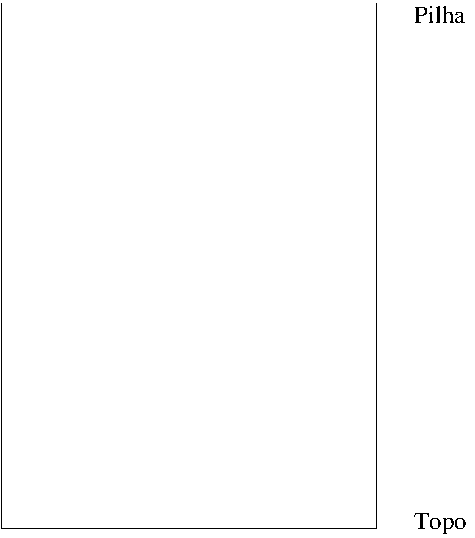
\includegraphics[width=0.5\textwidth]{figs/pilha0}
    \end{center}
\end{frame}

%%%%%%%%%%%%%%%%%%%%%%%%%%%%%%%%%%%%%%%%%%%%%%%%%%%%%%%%%%%%
\begin{frame}[fragile]{O que acontece na memória}
    Quando \cod{f2(2, 3)} é invocada, as variáveis locais de \cod{f2} são alocadas no topo da pilha.
    \begin{center}
        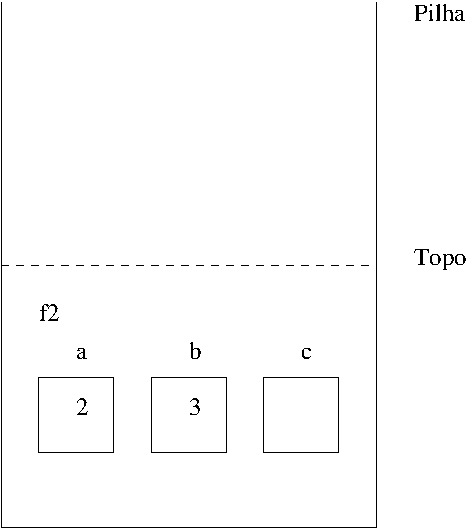
\includegraphics[width=0.5\textwidth]{figs/pilha1}
    \end{center}
\end{frame}

%%%%%%%%%%%%%%%%%%%%%%%%%%%%%%%%%%%%%%%%%%%%%%%%%%%%%%%%%%%%
\begin{frame}[fragile]{O que acontece na memória}
    A função \cod{f2} invoca a função \cod{f1(b, a)} e as variáveis locais desta são alocadas no topo da pilha, sobre as de \cod{f2}.
    \begin{center}
        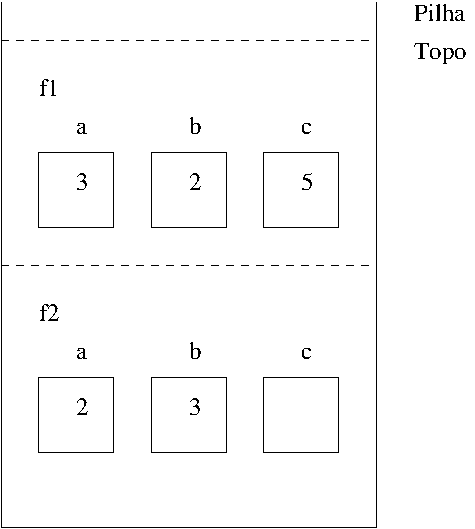
\includegraphics[width=0.5\textwidth]{figs/pilha2}
    \end{center}
\end{frame}

%%%%%%%%%%%%%%%%%%%%%%%%%%%%%%%%%%%%%%%%%%%%%%%%%%%%%%%%%%%%
\begin{frame}[fragile]{O que acontece na memória}
    A função \cod{f1} termina, devolvendo 10. As variáveis locais de \cod{f1} são removidas da pilha.
    \begin{center}
        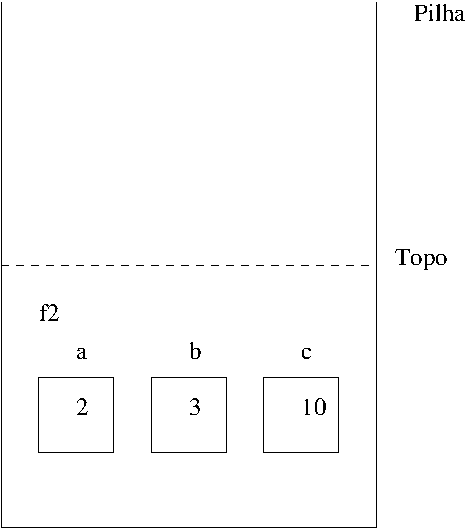
\includegraphics[width=0.5\textwidth]{figs/pilha3}
    \end{center}
\end{frame}

%%%%%%%%%%%%%%%%%%%%%%%%%%%%%%%%%%%%%%%%%%%%%%%%%%%%%%%%%%%%
\begin{frame}[fragile]{O que acontece na memória}
    Finalmente, \cod{f2} termina a sua execução devolvendo 10. Suas variáveis locais são removidas da pilha.
    \begin{center}
        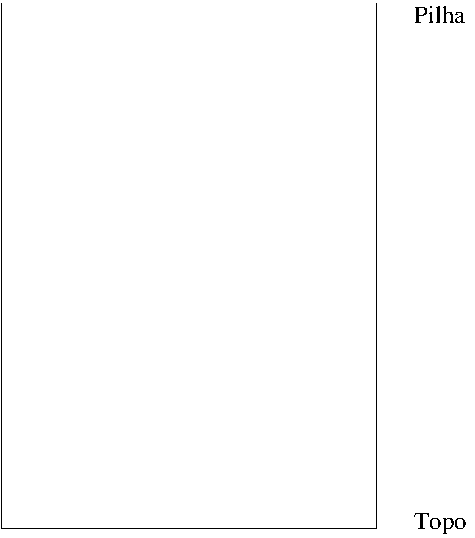
\includegraphics[width=0.5\textwidth]{figs/pilha0}
    \end{center}
\end{frame}

%%%%%%%%%%%%%%%%%%%%%%%%%%%%%%%%%%%%%%%%%%%%%%%%%%%%%%%%%%%%
\begin{frame}[fragile]{O que acontece na memória}

    No caso de chamadas recursivas para uma mesma função, é como se cada chamada correspondesse a uma função distinta.
    \begin{itemize}[<+->]
        \item As execuções das chamadas de funções recursivas são feitas na pilha, assim como qualquer função.
        \item O último conjunto de variáveis alocadas na pilha, que está no topo, corresponde às variáveis da última chamada da função.
        \item Quando termina a execução de uma chamada da função, as variáveis locais desta são removidas da pilha.
        \item Sem uma condição de parada, o algoritmo não para de chamar a si mesmo, até estourar a capacidade da pilha.
    \end{itemize}
\end{frame}

%%%%%%%%%%%%%%%%%%%%%%%%%%%%%%%%%%%%%%%%%%%%%%%%%%%%%%%%%%%%%%
\begin{frame}[fragile]{Usando recursão em programação}

    Considere novamente a solução recursiva para se calcular o fatorial e assuma que seja feito a chamada \cod{fatorial(4)}.
    \begin{minted}{c}
        long int fatorial(int n) {
            long int r, x;

            /* caso base: */
            if (n == 1)
                return 1;
            else {
                /* sabendo o fatorial de n-1: */
                x = n-1;
                r = fatorial(x);
                /* calculamos o fatorial de n: */
                return n * r;
            }
        }
    \end{minted}
\end{frame}

%%%%%%%%%%%%%%%%%%%%%%%%%%%%%%%%%%%%%%%%%%%%%%%%%%%%%%%%%%%%
\begin{frame}[fragile]{O que acontece na memória}

    \begin{itemize}[<+->]
        \item Cada chamada à função \cod{fatorial} cria novas variáveis locais de mesmo nome (\cod{n}, \cod{x} e \cod{r}).
        \item Portanto, várias variáveis \cod{n}, \cod{x} e \cod{r} podem existir em um dado momento.
        \item Em um dado instante, o nome \cod{n} (ou \cod{r}, ou \cod{x}) refere-se à variável local ao corpo da função que está sendo executada naquele instante.
    \end{itemize}
\end{frame}

%%%%%%%%%%%%%%%%%%%%%%%%%%%%%%%%%%%%%%%%%%%%%%%%%%%%%%%%%%%%
\begin{frame}[fragile]{O que acontece na memória}

    Estado da pilha de execução para \cod{fatorial(4)}:
    \begin{center}
        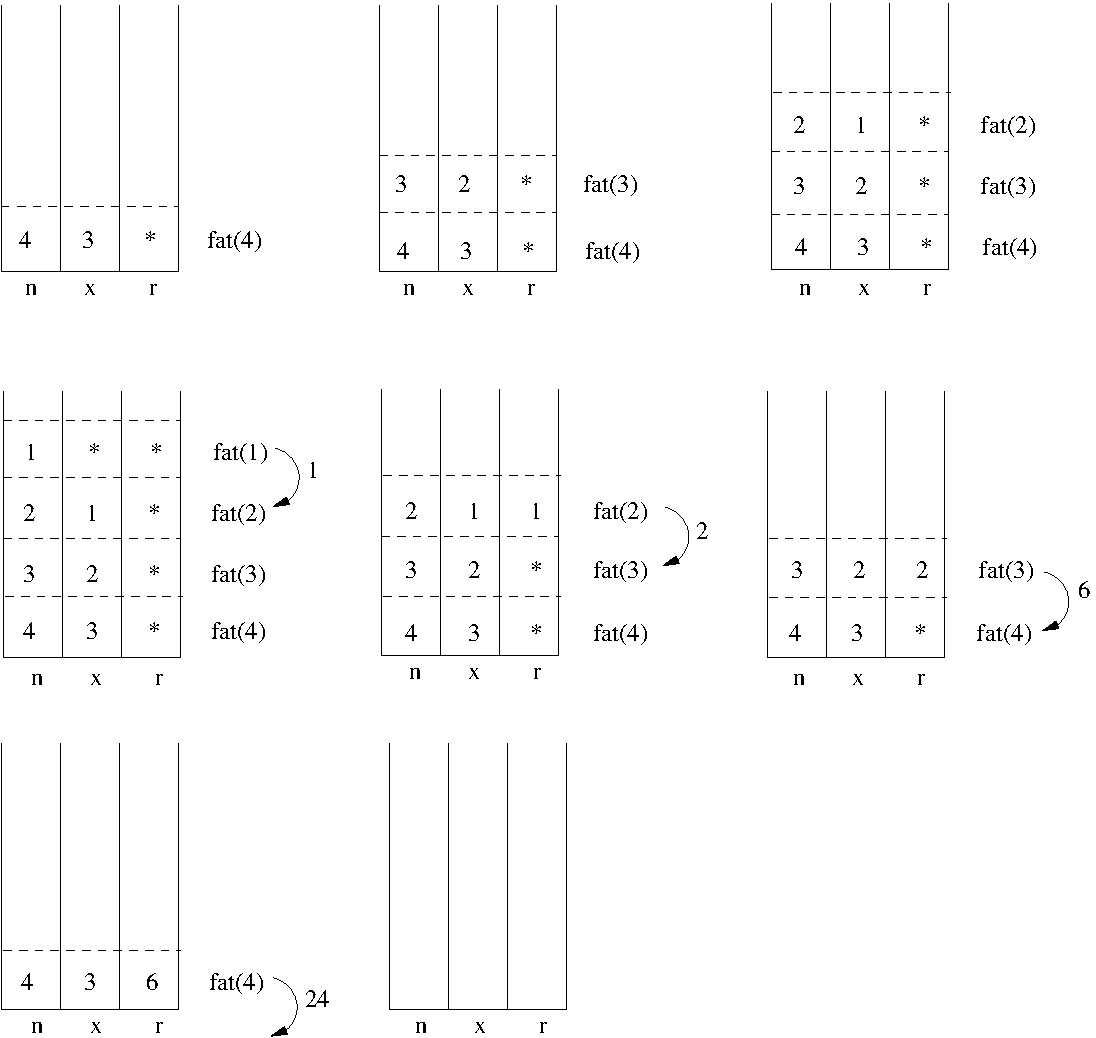
\includegraphics[width=0.7\textwidth]{figs/fatorial}
    \end{center}
\end{frame}

%%%%%%%%%%%%%%%%%%%%%%%%%%%%%%%%%%%%%%%%%%%%%%%%%%%%%%%%%%%%
\begin{frame}[fragile]{O que acontece na memória}

    \begin{itemize}
        \item É claro que as variáveis \cod{r} e \cod{x} são desnecessárias.
        \item E você também deveria testar se \cod{n} não é negativo!
    \end{itemize}

    \begin{minted}{c}
        long int fatorial(int n) {
            if (n <= 1)
                return 1;
            else
                return n * fatorial(n-1);
        }
    \end{minted}

    \pause

    \begin{minted}{c}
        long int fatorial(int n) {
            if (n <= 1)
                return 1;
            return n * fatorial(n-1);
        }
    \end{minted}
\end{frame}

%%%%%%%%%%%%%%%%%%%%%%%%%%%%%%%%%%%%%%%%%%%%%%%%%%%%%%%%%%%%
%%%%%%%%%%%%%%%%%%%%%%%%%%%%%%%%%%%%%%%%%%%%%%%%%%%%%%%%%%%%
%%%%%%%%%%%%%%%%%%%%%%%%%%%%%%%%%%%%%%%%%%%%%%%%%%%%%%%%%%%%
%%%%%%%%%%%%%%%%%%%%%%%%%%%%%%%%%%%%%%%%%%%%%%%%%%%%%%%%%%%%
%%%%%%%%%%%%%%%%%%%%%%%%%%%%%%%%%%%%%%%%%%%%%%%%%%%%%%%%%%%%
%%%%%%%%%%%%%%%%%%%%%%%%%%%%%%%%%%%%%%%%%%%%%%%%%%%%%%%%%%%%

\section{Recursão $\times$ Iteração}

%%%%%%%%%%%%%%%%%%%%%%%%%%%%%%%%%%%%%%%%%%%%%%%%%%%%%%%%%%%%
\begin{frame}[fragile]{Recursão $\times$ Iteração}

    \begin{itemize}[<+->]
        \item Soluções recursivas são geralmente mais concisas que as iterativas.
        \item Soluções iterativas em geral têm a memória limitada enquanto as recursivas, não.
        \item Cópia dos parâmetros a cada chamada recursiva é um custo adicional para as soluções recursivas.
    \end{itemize}
\end{frame}

%%%%%%%%%%%%%%%%%%%%%%%%%%%%%%%%%%%%%%%%%%%%%%%%%%%%%%%%%%%%
\begin{frame}[fragile]{Recursão $\times$ Iteração}

    No caso do cálculo do fatorial, uma solução iterativa é mais eficiente. Por quê?
    \begin{minted}{c}
        long int fatorial(int n) {
            long int result = 1;
            int i;

            for (i = 1; i <= n; i++)
                result = result * i;

            return r;
        }
    \end{minted}
\end{frame}

%%%%%%%%%%%%%%%%%%%%%%%%%%%%%%%%%%%%%%%%%%%%%%%%%%%%%%%%%%%%
%%%%%%%%%%%%%%%%%%%%%%%%%%%%%%%%%%%%%%%%%%%%%%%%%%%%%%%%%%%%
%%%%%%%%%%%%%%%%%%%%%%%%%%%%%%%%%%%%%%%%%%%%%%%%%%%%%%%%%%%%

\subsection{Exemplo: números de Fibonacci}

%%%%%%%%%%%%%%%%%%%%%%%%%%%%%%%%%%%%%%%%%%%%%%%%%%%%%%%%%%%%%%
\begin{frame}[fragile]{Recursão com várias chamadas}

    \begin{itemize}[<+->]
        \item Não há necessidade da função recursiva ter apenas uma chamada para si própria.
        \item A função pode fazer várias chamadas para si própria.
        \item A função pode ainda fazer chamadas recursivas indiretas: a função 1, por exemplo, chama uma outra função 2 que por sua vez chama a função 1.
    \end{itemize}
\end{frame}

%%%%%%%%%%%%%%%%%%%%%%%%%%%%%%%%%%%%%%%%%%%%%%%%%%%%%%%%%%%%%
\begin{frame}[fragile]{Fibonacci}

    \begin{itemize}
        \item A série de Fibonacci é a seguinte: $1, 1, 2, 3, 5, 8, 13, 21, \ldots$.
        \item Queremos determinar qual é o $n$-ésimo número da série, que denotaremos por $F(n)$.
        \item Como descrever o $n$-ésimo número de Fibonacci de forma recursiva?
    \end{itemize}
\end{frame}

%%%%%%%%%%%%%%%%%%%%%%%%%%%%%%%%%%%%%%%%%%%%%%%%%%%%%%%%%%%%%
\begin{frame}[fragile]{Fibonacci}

    \begin{itemize}
        \item No caso base, temos: se $n = 1$ ou $n = 2$, então $F(n) = 1$.
        \item Sabendo casos anteriores podemos computar $F(n)$:
        $$ F(n) = F(n-1) + F(n-2) \enspace .$$
    \end{itemize}
\end{frame}

%%%%%%%%%%%%%%%%%%%%%%%%%%%%%%%%%%%%%%%%%%%%%%%%%%%%%%%%%%%%%
\begin{frame}[fragile]{Fibonacci: algoritmo em C}

    A definição anterior é traduzida diretamente em um algoritmo em C:
    \begin{minted}{c}
        long int fibonacci(int n) {
            if (n <= 2)
                return 1;

            return fibonacci(n-1) + fibonacci(n-2);
        }
    \end{minted}
\end{frame}

%%%%%%%%%%%%%%%%%%%%%%%%%%%%%%%%%%%%%%%%%%%%%%%%%%%%%%%%%%%%%%
%%%%%%%%%%%%%%%%%%%%%%%%%%%%%%%%%%%%%%%%%%%%%%%%%%%%%%%%%%%%%%
%%%%%%%%%%%%%%%%%%%%%%%%%%%%%%%%%%%%%%%%%%%%%%%%%%%%%%%%%%%%%%

\subsection{Exemplo: cálculo de potências}

%%%%%%%%%%%%%%%%%%%%%%%%%%%%%%%%%%%%%%%%%%%%%%%%%%%%%%%%%%%%%%
\begin{frame}[fragile]{Cálculo de potências}

    Suponha que temos que calcular $x^n$ para $n$ inteiro positivo.

    Como calcular de forma recursiva?
    \pause

    $x^n$ é:
    \begin{itemize}
        \item 1, se $n=0$.
        \item $x x^{n-1}$, caso contrário.
    \end{itemize}
\end{frame}

%%%%%%%%%%%%%%%%%%%%%%%%%%%%%%%%%%%%%%%%%%%%%%%%%%%%%%%%%%%%%%
\begin{frame}[fragile]{Cálculo de Potências}

    \begin{minted}{c}
        long int pot(long int x, long int n) {
            if (n == 0)
                return 1;

            return x * pot(x, n-1);
        }
    \end{minted}
\end{frame}

%%%%%%%%%%%%%%%%%%%%%%%%%%%%%%%%%%%%%%%%%%%%%%%%%%%%%%%%%%%%%%
\begin{frame}[fragile]{Cálculo de Potências}

    Neste caso a solução iterativa é mais eficiente:

    \begin{minted}{c}
        long int pot(long int x, long int n) {
            long int result = 1, i;

            for (i = 1; i <= n; i++)
                result = result * x;

            return result;
        }
    \end{minted}
    \pause

    \begin{itemize}
        \item O laço é executado $n$ vezes.
        \item Na solução recursiva são feitas $n$ chamadas recursivas, mas tem-se o custo adicional para criação/remoção de variáveis locais na pilha.
    \end{itemize}
\end{frame}

%%%%%%%%%%%%%%%%%%%%%%%%%%%%%%%%%%%%%%%%%%%%%%%%%%%%%%%%%%%%%%
\begin{frame}[fragile]{Cálculo de Potências}

    Mas e se definirmos a potência de forma diferente?
    \pause

    $x^n$ é:
    \begin{itemize}[<+->]
        \item se $n=0$, então $x^n = 1$.
        \item se $n > 0$ e $n$ é par, então $x^n = (x^{n/2})^2$.
        \item se $n > 0$ e $n$ é ímpar, então $x^n = x(x^{(n-1)/2})^2$.
    \end{itemize}

    \pause
    Note que aqui também definimos a solução do caso maior em termos de casos menores.
\end{frame}

%%%%%%%%%%%%%%%%%%%%%%%%%%%%%%%%%%%%%%%%%%%%%%%%%%%%%%%%%%%%%%
\begin{frame}[fragile]{Cálculo de Potências}

    Este algoritmo é mais eficiente do que o iterativo. Por quê?

    Quantas chamadas recursivas o algoritmo pode fazer?

    \begin{minted}[fontsize=\scriptsize]{c}
        long int pot(long int x, long int n) {
            long int aux;

            if (n == 0)
                return 1;

            else if (n % 2 == 0) {
                aux = pot(x, n/2);
                return aux * aux;
            }

            else {
                aux = pot(x, (n-1)/2);
                return x * aux * aux;
            }
        }
    \end{minted}
\end{frame}

%%%%%%%%%%%%%%%%%%%%%%%%%%%%%%%%%%%%%%%%%%%%%%%%%%%%%%%%%%%%%%
\begin{frame}[fragile]{Cálculo de Potências}

    \begin{itemize}[<+->]
        \item No algoritmo anterior, a cada chamada recursiva o valor de $n$ é dividido por 2. Ou seja, a cada chamada recursiva, o valor de $n$ decai para pelo menos a metade.
        \item Usando divisões inteiras faremos no máximo $\lceil (\log_2 n) \rceil +1$ chamadas recursivas.
        \item Enquanto isso, o algoritmo iterativo executa o laço $n$ vezes.
    \end{itemize}
\end{frame}

%%%%%%%%%%%%%%%%%%%%%%%%%%%%%%%%%%%%%%%%%%%%%%%%%%%%%%%%%%%%%
%%%%%%%%%%%%%%%%%%%%%%%%%%%%%%%%%%%%%%%%%%%%%%%%%%%%%%%%%%%%%
%%%%%%%%%%%%%%%%%%%%%%%%%%%%%%%%%%%%%%%%%%%%%%%%%%%%%%%%%%%%%

\subsection{Torres de Hanoi}

%%%%%%%%%%%%%%%%%%%%%%%%%%%%%%%%%%%%%%%%%%%%%%%%%%%%%%%%%%%%%%
\begin{frame}[fragile]{Torres de Hanoi}
    \begin{center}
        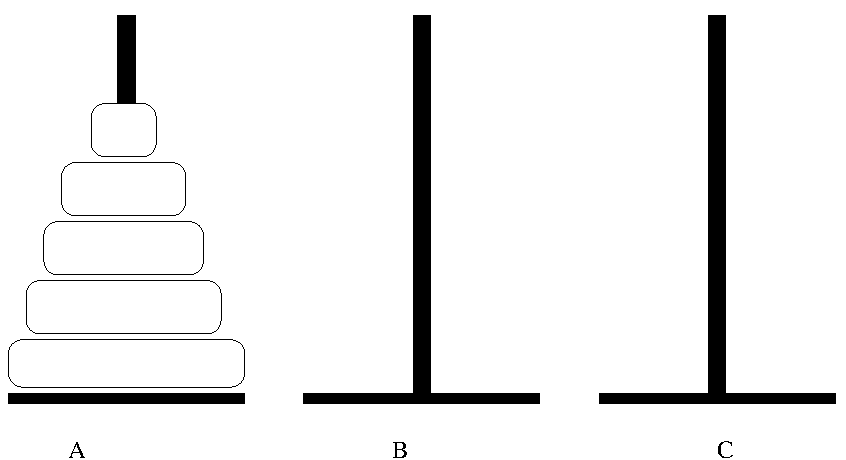
\includegraphics[width=\textwidth]{figs/hanoi}
    \end{center}
\end{frame}

%%%%%%%%%%%%%%%%%%%%%%%%%%%%%%%%%%%%%%%%%%%%%%%%%%%%%%%%%%%%%%
\begin{frame}[fragile]{Torres de Hanoi}

    \begin{itemize}[<+->]
        \item Inicialmente temos 5 discos de diâmetros diferentes na estaca A.
        \item O problema das torres de Hanoi consiste em transferir os cinco discos da estaca A para a estaca C (pode-se usar a estaca B como auxiliar).
        \item Porém deve-se respeitar as seguintes regras:
        \begin{itemize}
            \item Apenas o disco do topo de uma estaca pode ser movido.
            \item Nunca um disco de diâmetro maior pode ficar sobre um disco de diâmetro menor.
        \end{itemize}
    \end{itemize}
\end{frame}

%%%%%%%%%%%%%%%%%%%%%%%%%%%%%%%%%%%%%%%%%%%%%%%%%%%%%%%%%%%%%%
\begin{frame}[fragile]{Torres de Hanoi}

    \begin{itemize}
        \item Vamos considerar o problema geral onde há $n$ discos.
        \item Vamos usar indução para obtermos um algoritmo para este problema.
    \end{itemize}
\end{frame}

%%%%%%%%%%%%%%%%%%%%%%%%%%%%%%%%%%%%%%%%%%%%%%%%%%%%%%%%%%%%%%
\begin{frame}[fragile]{Torres de Hanoi}

    \begin{itemize}[<+->]
        \item Base: $n=1$. Neste caso temos apenas um disco. Basta mover este disco da estaca A para a estaca C.
        \item Hipótese: Sabemos como resolver o problema quando há $n-1$ discos.
        \item Passo: Devemos resolver o problema para $n$ discos.
        \begin{itemize}
            \item Por hipótese de indução, sabemos mover os $n-1$ primeiros discos da estaca {\bf A} para {\bf B} usando {\bf C} como auxiliar.
            \item Depois de movermos estes $n-1$ discos, movemos o maior disco (que continua na estaca {\bf A}) para a estaca {\bf C}.
            \item Novamente pela hipótese de indução, sabemos mover os $n-1$ discos da estaca {\bf B} para {\bf C} usando {\bf A} como auxiliar.
        \end{itemize}
        \item Com isso temos uma solução para o caso onde há $n$ discos.
        \item A indução nos fornece um algoritmo e ainda por cima temos uma demonstração formal de que ele funciona!
    \end{itemize}
\end{frame}

%%%%%%%%%%%%%%%%%%%%%%%%%%%%%%%%%%%%%%%%%%%%%%%%%%%%%%%%%%%%%%
\begin{frame}[fragile]{Torres de Hanoi: algoritmo}

    Problema: Mover $n$ discos de {\bf A} para {\bf C}.

    \begin{enumerate}[<+->]
        \item Se $n=1$, então mova o único disco de {\bf A} para {\bf C} e pare.
        \item Caso contrário ($n > 1$) desloque de forma recursiva os $n-1$ primeiros discos de {\bf A} para {\bf B}, usando {\bf C} como auxiliar.
        \item Mova o último disco de {\bf A} para {\bf C}.
        \item Mova, de forma recursiva, os $n-1$ discos de {\bf B} para {\bf C}, usando {\bf A} como auxiliar.
    \end{enumerate}
\end{frame}

%%%%%%%%%%%%%%%%%%%%%%%%%%%%%%%%%%%%%%%%%%%%%%%%%%%%%%%%%%%%%%
\begin{frame}[fragile]{Torres de Hanoi: algoritmo}

    A função que computa a solução (em C) terá o seguinte protótipo:

    \begin{minted}{c}
        void hanoi(int n, char estacaInicio, char estacaFim, char estacaAux);
    \end{minted}

    É passado como parâmetro o número de discos a ser movido ({\bf n}) e três caracteres indicando de onde os discos serão movidos ({\bf estacaInicio}), para onde devem ser movidos ({\bf estacaFim}) e qual é a estaca auxiliar ({\bf estacaAux}).
\end{frame}

%%%%%%%%%%%%%%%%%%%%%%%%%%%%%%%%%%%%%%%%%%%%%%%%%%%%%%%%%%%%%%
\begin{frame}[fragile]{Torres de Hanoi: algoritmo}

    A função que computa a solução é:

    \begin{minted}[fontsize=\scriptsize]{c}
        void hanoi(int n, char estacaInicio, char estacaFim, char estacaAux) {
            if (n == 1) {
                /* Caso base: move o único disco diretamente */
                printf("Mova disco %d de %c para %c.\n", n, estacaInicio, estacaFim);
            } else {
                /* Move n-1 discos de Inicio para Aux usando Fim de auxiliar: */
                hanoi(n-1, estacaInicio, estacaAux, estacaFim);

                /* Move o maior disco para estacaFim: */
                printf("Mova disco %d de %c para %c.\n", n, estacaInicio, estacaFim);

                /* Move os n-1 discos de Aux para Fim usando Ini de auxiliar: */
                hanoi(n-1, estacaAux, estacaFim, estacaInicio);
            }
        }
    \end{minted}
\end{frame}

%%%%%%%%%%%%%%%%%%%%%%%%%%%%%%%%%%%%%%%%%%%%%%%%%%%%%%%%%%%%%%
\begin{frame}[fragile]{Torres de Hanoi: algoritmo}

    \begin{minted}[fontsize=\scriptsize]{c}
        #include <stdio.h>

        void hanoi(int n, char estacaInicio, char estacaFim, char estacaAux);

        int main() {
            hanoi(4, 'A', 'C', 'B');
            return 0;
        }

        void hanoi(int n, char estacaInicio, char estacaFim, char estacaAux) {
            if (n == 1)
                printf("Mova disco %d de %c para %c.\n", n, estacaInicio, estacaFim);
            else {
                hanoi(n-1, estacaInicio, estacaAux, estacaFim);
                printf("Mova disco %d de %c para %c.\n", n, estacaInicio, estacaFim);
                hanoi(n-1, estacaAux, estacaFim, estacaInicio);
            }
        }
    \end{minted}
\end{frame}

%%%%%%%%%%%%%%%%%%%%%%%%%%%%%%%%%%%%%%%%%%%%%%%%%%%%%%%%%%%%%%
%%%%%%%%%%%%%%%%%%%%%%%%%%%%%%%%%%%%%%%%%%%%%%%%%%%%%%%%%%%%%%
%%%%%%%%%%%%%%%%%%%%%%%%%%%%%%%%%%%%%%%%%%%%%%%%%%%%%%%%%%%%%%
%%%%%%%%%%%%%%%%%%%%%%%%%%%%%%%%%%%%%%%%%%%%%%%%%%%%%%%%%%%%%%
%%%%%%%%%%%%%%%%%%%%%%%%%%%%%%%%%%%%%%%%%%%%%%%%%%%%%%%%%%%%%%
%%%%%%%%%%%%%%%%%%%%%%%%%%%%%%%%%%%%%%%%%%%%%%%%%%%%%%%%%%%%%%

\section{Exercícios}

%%%%%%%%%%%%%%%%%%%%%%%%%%%%%%%%%%%%%%%%%%%%%%%%%%%%%%%%%%%%%%
\begin{frame}[fragile]{Exercício}

    O que será impresso pela chamada \cod{imprimir(5)?}
    \begin{minted}{c}
        void imprimir(int i) {
            int j;
            if (i > 0) {
                imprimir(i - 1);
                for (j = 1; j <= i; j++)
                    printf("*");
                printf("\n");
            }
        }
    \end{minted}
\end{frame}

%%%%%%%%%%%%%%%%%%%%%%%%%%%%%%%%%%%%%%%%%%%%%%%%%%%%%%%%%%%%%%
\begin{frame}[fragile]{Exercício}
    Mostre o estado da pilha de memória durante a execução da função \cod{fibonacci} com a chamada \cod{fibonacci(5)}.

    Qual versão é mais eficiente para se calcular o $n$-ésimo número de Fibonacci, a recursiva ou a iterativa? Justifique.
\end{frame}

%%%%%%%%%%%%%%%%%%%%%%%%%%%%%%%%%%%%%%%%%%%%%%%%%%%%%%%%%%%%%%
\begin{frame}{Exercício}
    Escreva uma função recursiva que, dado um número inteiro positivo $n$, imprima a representação binária de $n$
\end{frame}




\end{document}
